\section{Donantes de sangre}

La compatibilidad sanguínea es un importante avance científico que permite conocer si una persona (donante) puede entregar su sangre a otra (receptor) y que esta la reciba conformemente sin presentar rechazo.

\begin{center}
    \textit{Quien salva una vida es un héroe, quien salva diez es donante.}
\end{center}

Considere que la información de posibles donantes se encuentra guardada en una lista de tuplas de la forma \texttt{nombre, tipo de sangre}. También se tiene una lista ordenada de los tipos de sangre (para obtener un índice numérico) y finalmente una matriz de datos de donantes y receptores.

\begin{figure}[H]
    \centering
    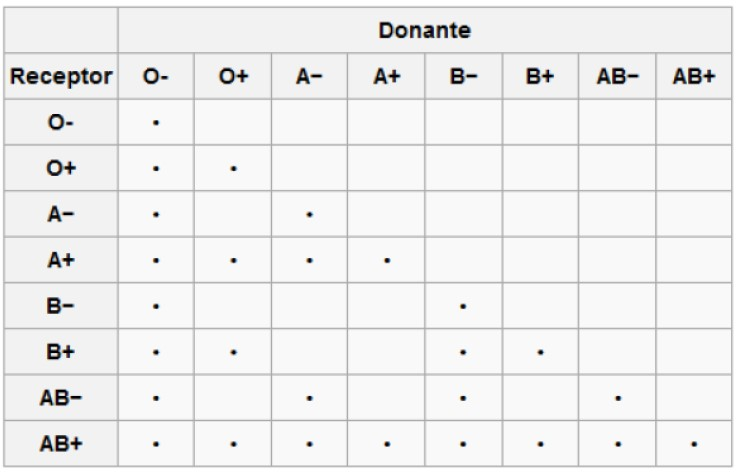
\includegraphics[scale=0.6]{Guia/sangre.jpg}
    \caption{Matriz de datos para donantes y receptores}
\end{figure}

Un famoso tutor de programación ha tenido un accidente y para salvar su vida es necesario realizarle una transfusión sanguínea. El problema es que ese tutor es grupo B Rh -, el cual es sumamente escaso. Para buscar posibles donantes el tutor necesita que los buenos alumnos de programación IWI131 que van a estudiar a CIAC creen las siguientes funciones.

\begin{itemize}
    \item[a.] \texttt{tipos\_donantes(tipo\_sangre,matriz,sangres)} que reciba un string con un  tipo de sangre, la matriz (lista de listas) anterior de posibles donadores o receptores y la lista \texttt{sangres} que contiene ordenados los tipos sanguíneos. Esta función debe retornar una lista de strings con los posibles grupos sanguíneos que pueden donar a \texttt{tipo\_sangre}.
    \item[b.] \texttt{donantes(gente, tipo)} que reciba una lista de gente (de la forma nombre y tipo de sangre) además de un string \texttt{tipo} que contiene la información del grupo sanguíneo del receptor. Esta función retorna una lista de tuplas (de la forma nombre y tipo sanguíneo) con todas las posibles personas que pueden donar al tipo sanguíneo solicitado.
    \item[c.] \texttt{sobrevive(max\_donacion,requerida,tipo\_sanguineo)} que recibe como parámetros \\ \texttt{max\_donacion} que corresponde a la cantidad máxima de sangre que puede donar un individuo, y \texttt{requerida} que corresponde a la cantidad de sangre que se necesita recolectar. En caso de que la cantidad de donantes sea suficiente para reunir la cantidad de sangre requerida la función debe retornar \texttt{True}, en caso contrario retornará \texttt{False}.
\end{itemize}